% This is "sig-alternate.tex" V2.1 April 2013
% This file should be compiled with V2.5 of "sig-alternate.cls" May 2012
%
% This example file demonstrates the use of the 'sig-alternate.cls'
% V2.5 LaTeX2e document class file. It is for those submitting
% articles to ACM Conference Proceedings WHO DO NOT WISH TO
% STRICTLY ADHERE TO THE SIGS (PUBS-BOARD-ENDORSED) STYLE.
% The 'sig-alternate.cls' file will produce a similar-looking,
% albeit, 'tighter' paper resulting in, invariably, fewer pages.
%
% ----------------------------------------------------------------------------------------------------------------
% This .tex file (and associated .cls V2.5) produces:
%       1) The Permission Statement
%       2) The Conference (location) Info information
%       3) The Copyright Line with ACM data
%       4) NO page numbers
%
% as against the acm_proc_article-sp.cls file which
% DOES NOT produce 1) thru' 3) above.
%
% Using 'sig-alternate.cls' you have control, however, from within
% the source .tex file, over both the CopyrightYear
% (defaulted to 200X) and the ACM Copyright Data
% (defaulted to X-XXXXX-XX-X/XX/XX).
% e.g.
% \CopyrightYear{2007} will cause 2007 to appear in the copyright line.
% \crdata{0-12345-67-8/90/12} will cause 0-12345-67-8/90/12 to appear in the copyright line.
%
% ---------------------------------------------------------------------------------------------------------------
% This .tex source is an example which *does* use
% the .bib file (from which the .bbl file % is produced).
% REMEMBER HOWEVER: After having produced the .bbl file,
% and prior to final submission, you *NEED* to 'insert'
% your .bbl file into your source .tex file so as to provide
% ONE 'self-contained' source file.
%
% ================= IF YOU HAVE QUESTIONS =======================
% Questions regarding the SIGS styles, SIGS policies and
% procedures, Conferences etc. should be sent to
% Adrienne Griscti (griscti@acm.org)
%
% Technical questions _only_ to
% Gerald Murray (murray@hq.acm.org)
% ===============================================================
%
% For tracking purposes - this is V2.0 - May 2012

\documentclass{sig-alternate-05-2015}
\usepackage{placeins}
\usepackage{epstopdf}


\begin{document}

% Copyright
%\setcopyright{acmcopyright}
%\setcopyright{acmlicensed}
%\setcopyright{rightsretained}
%\setcopyright{usgov}
%\setcopyright{usgovmixed}
%\setcopyright{cagov}
%\setcopyright{cagovmixed}


%
% --- Author Metadata here ---
%\conferenceinfo{WOODSTOCK}{'97 El Paso, Texas USA}
%\CopyrightYear{2007} % Allows default copyright year (20XX) to be over-ridden - IF NEED BE.
%\crdata{0-12345-67-8/90/01}  % Allows default copyright data (0-89791-88-6/97/05) to be over-ridden - IF NEED BE.
% --- End of Author Metadata ---

\title{Recommendation Algorithms for User First Booking on Airbnb}

%
% You need the command \numberofauthors to handle the 'placement
% and alignment' of the authors beneath the title.
%
% For aesthetic reasons, we recommend 'three authors at a time'
% i.e. three 'name/affiliation blocks' be placed beneath the title.
%
% NOTE: You are NOT restricted in how many 'rows' of
% "name/affiliations" may appear. We just ask that you restrict
% the number of 'columns' to three.
%
% Because of the available 'opening page real-estate'
% we ask you to refrain from putting more than six authors
% (two rows with three columns) beneath the article title.
% More than six makes the first-page appear very cluttered indeed.
%
% Use the \alignauthor commands to handle the names
% and affiliations for an 'aesthetic maximum' of six authors.
% Add names, affiliations, addresses for
% the seventh etc. author(s) as the argument for the
% \additionalauthors command.
% These 'additional authors' will be output/set for you
% without further effort on your part as the last section in
% the body of your article BEFORE References or any Appendices.

\numberofauthors{3} %  in this sample file, there are a *total*
% of EIGHT authors. SIX appear on the 'first-page' (for formatting
% reasons) and the remaining two appear in the \additionalauthors section.
%
\author{
% You can go ahead and credit any number of authors here,
% e.g. one 'row of three' or two rows (consisting of one row of three
% and a second row of one, two or three).
%
% The command \alignauthor (no curly braces needed) should
% precede each author name, affiliation/snail-mail address and
% e-mail address. Additionally, tag each line of
% affiliation/address with \affaddr, and tag the
% e-mail address with \email.
%
% 1st. author
\alignauthor Zhao Wang \\
       \affaddr{Northeastern University}\\
       \affaddr{Seattle, WA}\\
       \email{\large wang.zhao2@husky.neu.edu}
% 2nd. author
\alignauthor Zerui Ma \\
      \affaddr{Northeastern University}\\
       \affaddr{Seattle, WA}\\
       \email{\large zeruima1989@gmail.com}
% 3rd. author
\alignauthor Heng Xu\\
       \affaddr{Northeastern University}\\
       \affaddr{Seattle, WA}\\
       \email{\large xu.he@husky.neu.edu}
}
% There's nothing stopping you putting the seventh, eighth, etc.
% author on the opening page (as the 'third row') but we ask,
% for aesthetic reasons that you place these 'additional authors'
% in the \additional authors block, viz.

% Just remember to make sure that the TOTAL number of authors
% is the number that will appear on the first page PLUS the
% number that will appear in the \additionalauthors section.

\maketitle
\begin{abstract}
In this paper, we aim to design an optimal recommendation algorithm to predict which country new users on Airbnb will make their first booking. A variety of methods including basic classifiers, ensemble methods, recommendation algorithms and 3-layer ensemble framework are used to solve this problem. To start off, some basic classifiers are used for error rate evaluations. Ensemble methods are then introduced to improve the performance of the weak learners. In addition, a recommendation algorithm based on collaborative filtering is designed to obtain a better performance. In order to further improve the result, a 3-layer ensemble framework that combines on basic classifiers and ensemble methods is introduced.
\end{abstract}


%
% The code below should be generated by the tool at
% http://dl.acm.org/ccs.cfm
% Please copy and paste the code instead of the example below. 
%
\begin{CCSXML}
<ccs2012>
 <concept>
  <concept_id>10010520.10010553.10010562</concept_id>
  <concept_desc>Computer systems organization~Embedded systems</concept_desc>
  <concept_significance>500</concept_significance>
 </concept>
 <concept>
  <concept_id>10010520.10010575.10010755</concept_id>
  <concept_desc>Computer systems organization~Redundancy</concept_desc>
  <concept_significance>300</concept_significance>
 </concept>
 <concept>
  <concept_id>10010520.10010553.10010554</concept_id>
  <concept_desc>Computer systems organization~Robotics</concept_desc>
  <concept_significance>100</concept_significance>
 </concept>
 <concept>
  <concept_id>10003033.10003083.10003095</concept_id>
  <concept_desc>Networks~Network reliability</concept_desc>
  <concept_significance>100</concept_significance>
 </concept>
</ccs2012>  
\end{CCSXML}



%
% End generated code
%

%
%  Use this command to print the description
%
\printccsdesc

% We no longer use \terms command
%\terms{Theory}

\keywords{Learning Algorithms; Classifier; Ensemble; Collaborative Filtering}

\section{Introduction}
Data mining is the process of discovering interesting patterns from massive amounts of data. As a knowledge discovery process, it typically involves data cleaning, data integration, data selection, data transformation, pattern discovery, pattern evaluation, and knowledge presentation\cite{data mining}. The science of learning plays a key role in the fields of data mining, statistics and artificial intelligence, intersecting with areas of engineering and other disciplines\cite{statistical}.  In a typical scenario, a quantitative or categorical outcome measurement is predicted based on a set of features.

Recommendation algorithms are a type of learning algorithms that are widely used on e-commerce websites.  They use customer interests as input to generate a list of recommended items. Most recommendation algorithms are designed for finding similar customers, then they aggregate items from similar customers, eliminates items the user has already purchased or rated, and recommends the remaining items to the user. The popular versions of these algorithms are collaborative filtering and cluster models. In collaborative filtering, the similarity of customers is measured by the cosine of the angle between the two vectors which represent users' interests\cite{analysis}. Using this algorithm to generate recommendations is computationally expensive, but it can be released by dimensionally reduction techniques\cite{collaborative}. To find the similar customers to the user, cluster models divide the customer base into many segments and treat the task as a classification problem\cite{clustering}.  Some algorithms classify users into multiple segments and describe the strength of each relationship\cite{cf}. In addition to grouping the user to the similar customers, other algorithms such as search-based methods and item-to-item collaborative filtering focus on finding similar items\cite{item2item}. Search- or content-based methods treat the recommendations problem as a search for related items\cite{massive}.

Nowadays, user experience has become an increasingly critical factor for a company to keep existing users and attract new users among various competitors. By building an effective recommendation system to predict where a new user will book his or her first travel destination, Airbnb can provide a personalized and unique experience for its new users, reduce the average first booking time, and gain a better understanding of the business demand. 


However, the main challenge here is that Airbnb does not have the travel history or other type of traveling data from new users. The only data available here are basic features such as age, gender, session log etc., which is basically like a white paper to a recommendation system. While a typical recommendation system might make recommendations based on a few strongly related features, the system designed here need to focus on correctly classifying similar users first, then trying to make recommendation with some relatively strong features. This is the primary reason we choose collaborative filtering as our first-step approach.

\section{Dataset Description}
In this section, the data sets used for the recommendation algorithms are introduced. The data are consisted of two parts: the first one is the list of users' first booking destinations as well as their personal information and web session records; the second is the aggregated public host information dataset sourced from the Airbnb site. By analyzing the statistics and features of the source data, we are able to have an overview of the entire data and decide how to process and apply the data for the recommendation algorithms.

\subsection{User data set}
In the list of user first booking file, each user is specified by a unique string id and each record contains multiple types of properties for that user, including account created time, age, sign up device, etc. Each field contains missing and inconsistent values which should be addressed before training the recommendation model. The users whose destination countries are unavailable (indicated as NDF) also need to be filtered out since those are the users we are going to predict where their destination countries are. The details of user properties are described as Table.\ref{table:users}.

\begin{table}[!htb]
\caption{User Data Statistics}
\label{table:users}
\begin{tabular}{|c|c|l|} \hline
field & type & description  \\ \hline                                                                                                                              
id & string & unique for each user \\ \hline                                                                                                                     
\shortstack{date\_account\\ \_created} & date & ~ \\ \hline                                                                                                                                             
\shortstack{timestamp\_first\\ \_active}  & timestampe & ~  \\ \hline                                                                                                                                          \shortstack{date\_first\\ \_booking} & date & ~ \\ \hline                                                                                                                                             
gender & categorical & \shortstack[l]{FEMALE, MALE, \\OTHER, unknown} \\ \hline                                                                                                                 
age & numerical & 1 to 150  \\ \hline                                                                                                                      
signup\_method  & categorical & basic, facebook, google  \\ \hline                                                                                                                       
signup\_flow & numerical & 0 to 25  \\ \hline                                                                                                                                  language & categorical & en, zh, fr, es, ko, de, etc.  \\ \hline                                                                                                              
affiliate\_channel  & categorical & \shortstack[l]{api, content, direct, etc}  \\ \hline
affiliate\_provider  & categorical & \shortstack[l]{bing, facebook, google, etc} \\ \hline
\shortstack{first\_affiliate\\ \_tracked} & categorical & \shortstack[l]{linked, local ops, \\ product, etc.} \\ \hline
signup\_app & categorical & Android, iOS, Moweb, Web \\ \hline
first\_device\_type & categorical & \shortstack[l]{Android Phone, iPad, \\ iPhone, Mac Desktop, etc.} \\ \hline
first\_browser  & categorical & \shortstack[l]{Chrome, Safari, Firefox, etc.} \\ 
\hline \end{tabular}
\end{table}

After dropping the records without specific destinations, the number of the users for each country are shown as Table.\ref{table:destination} described. The instances with specific destinations are the data we should focus on to build the predication model for new users. From the Table.\ref{table:destination} we conclude that most users choose U.S. as their first booking destination since Airbnb is a company in the U.S. There are quite a number of users traveling to the countries that are not listed in those specific countries (indicated as other).

\begin{table}[!htb]
\centering
\caption{Users First Booking Destination}
\label{table:destination}
\begin{tabular}{|c|c|l|} \hline
Destination Country & Population\\ \hline
AU & 537 \\ \hline
CA & 1425 \\ \hline
DE & 1059 \\ \hline
ES & 2243 \\ \hline
FR & 5013 \\ \hline
GB & 2318 \\ \hline
IT & 2827 \\ \hline
NL & 757 \\ \hline
PT & 217 \\ \hline
US &  62263 \\ \hline
other & 10075 \\
\hline\end{tabular}
\end{table}

The Figure.\ref{fig:age distribution} describes the age distribution of the users in the list. It can be seen that users between the age of 25-45 are more likely to travel. 

\begin{figure}[!htb]
\centering
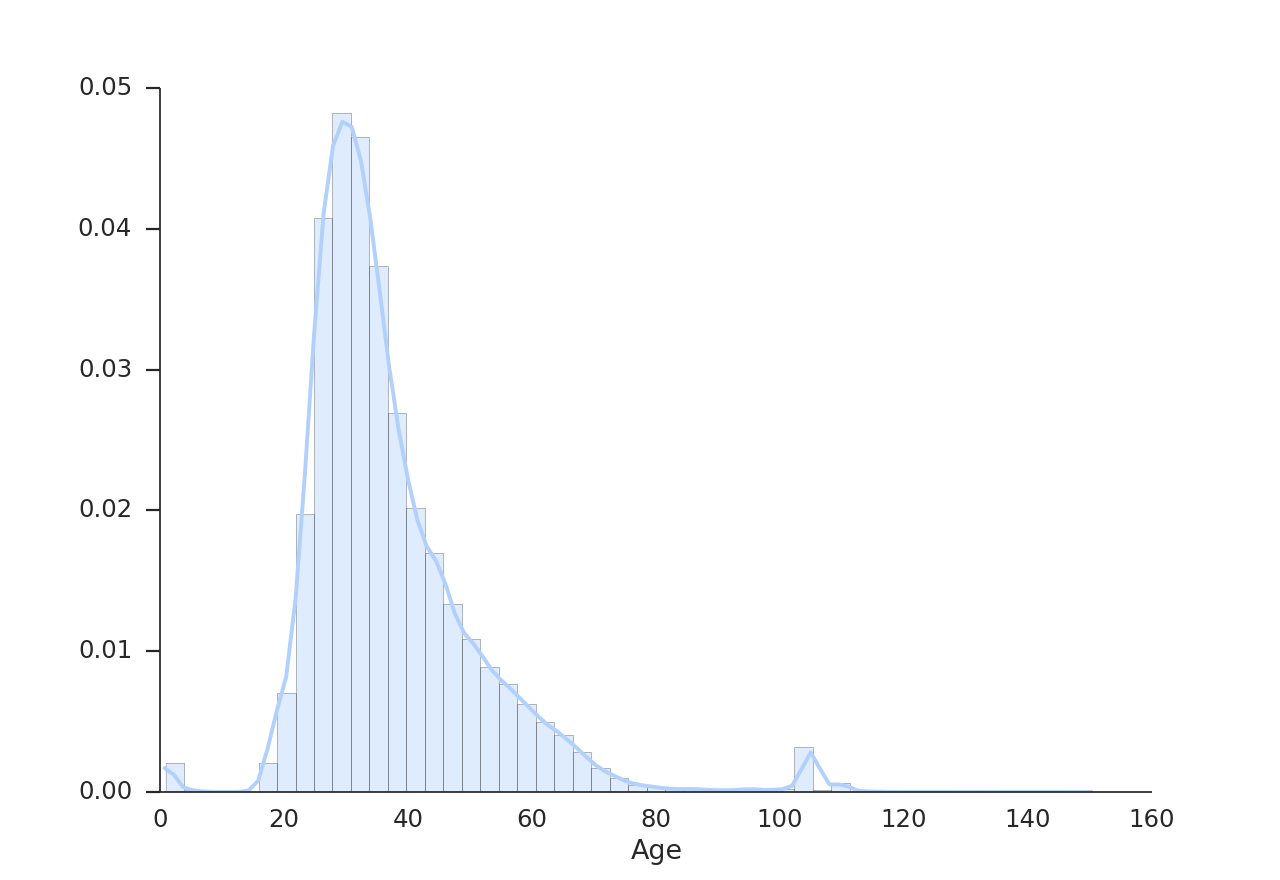
\includegraphics[height=2in, width=3in]{AgeDistribution}
\caption{Age Distribution for Users on Airbnb}
\label{fig:age distribution}
\end{figure}


\FloatBarrier
\subsection{Hosts data set}
The other data set contains more detailed information of host listings among 16 countries available on Airbnb. It covers almost all the countries corresponding to the new user data set, but listing data from PT(Portugal) is missing.

This listing data set contains most of the publicly available information on Airbnb. Lots of features such as listing price, listing rating score, host registration information and neighborhood etc., may help recommendation system identify better listings among target countries for new users. However, due to the limitation of the new user data, the recommendation on this part is most likely to be based on features weighted by common sense such as highest rated, best available price etc..

\begin{figure}[!htb]
\centering
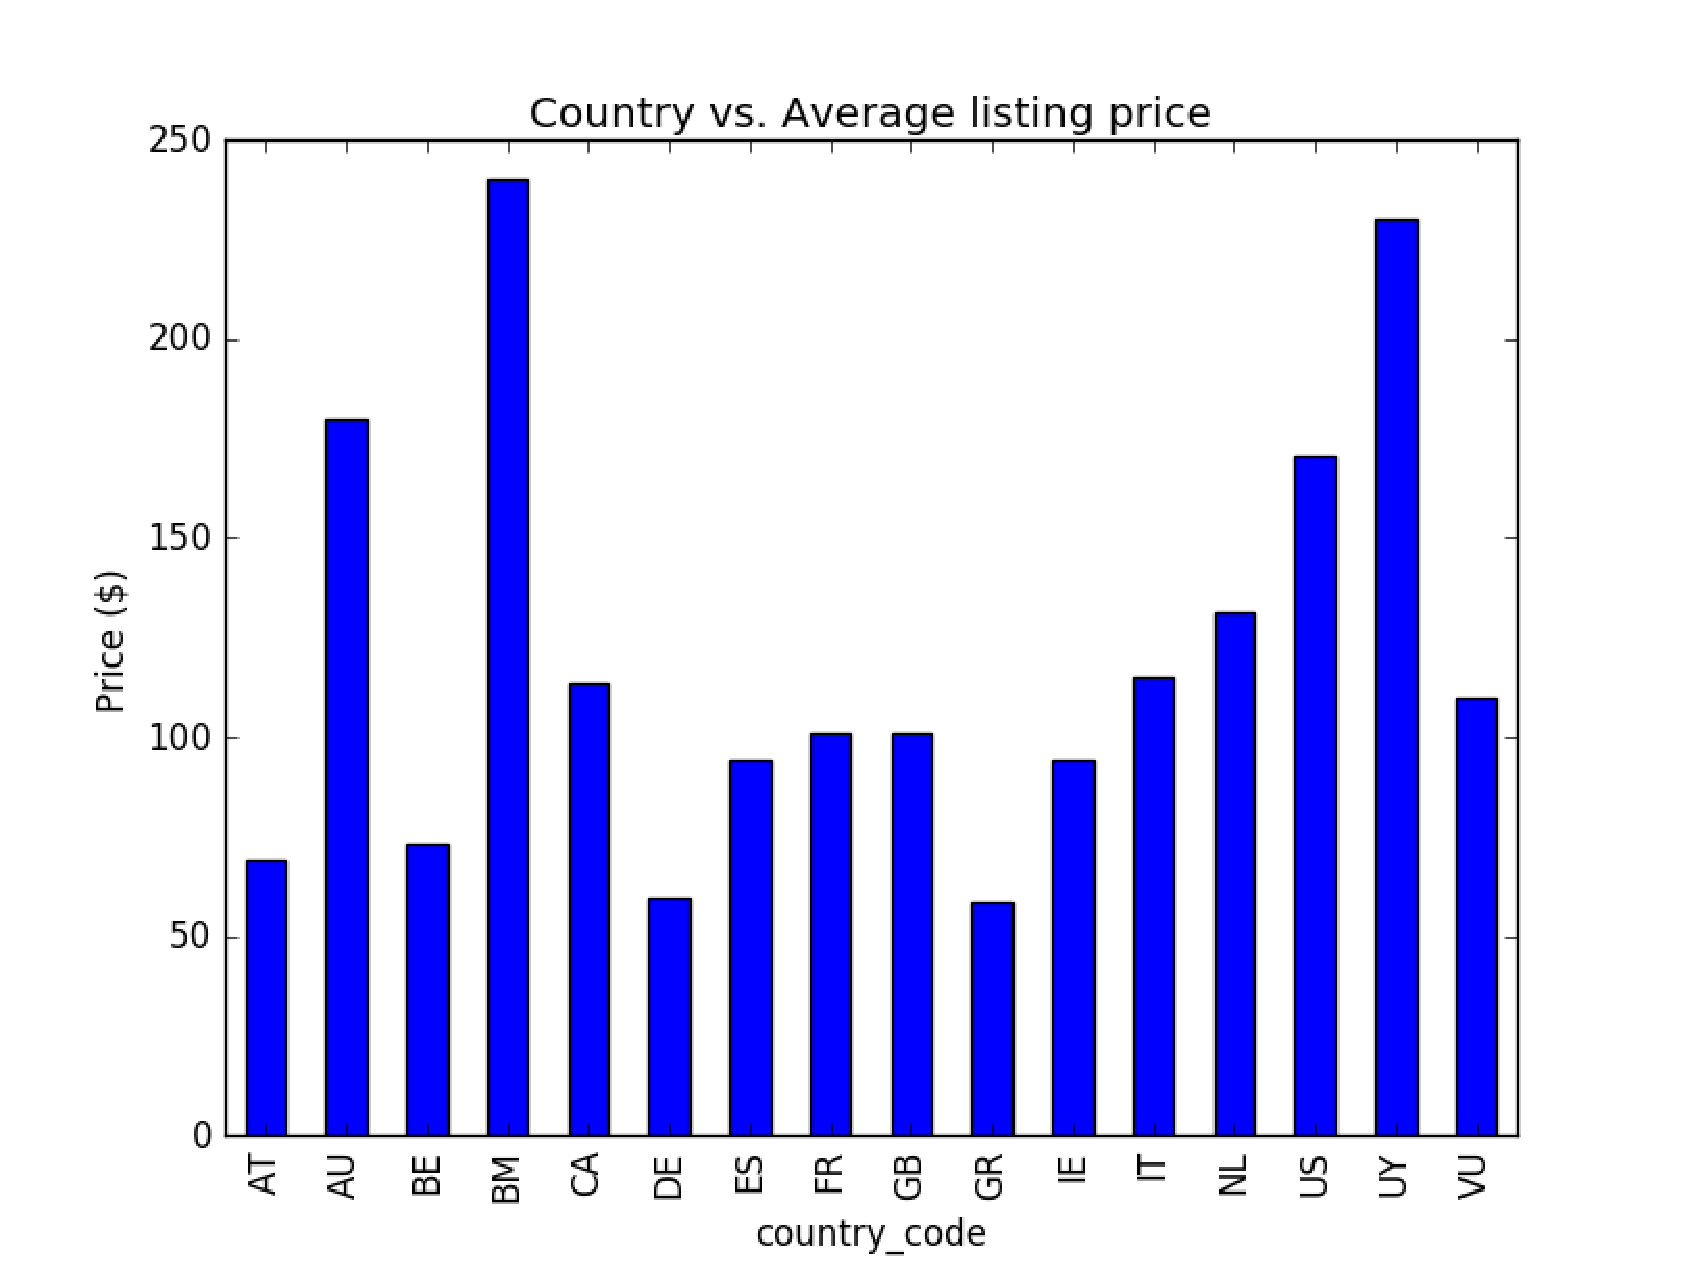
\includegraphics[height=2in, width=3in]{country-avgPrice}
\caption{Average price distribution among countries}
\end{figure}

Since listing price is showed in dollar, the average listing price distribution is influenced by currency exchange rate in some extent. In addition to this fact, the average listing price definitely reflects the popularity of these destination countries. BM(Bermuda) is a typical high-end vacation hot spot, but it is surprising to see UY(Uruguay) has such a high average price, maybe due to the fact that the retrieved UY listings is very limited. Other than these two countries, AU and US are the most expensive countries to go on Airbnb. It is interesting to see AU has a higher average listing price than US. A possible explanation for this could be the number of listings in US is much greater than AU's, thus competition over the host has lowered the average listing price in the US.

\begin{figure}[!htb]
\centering
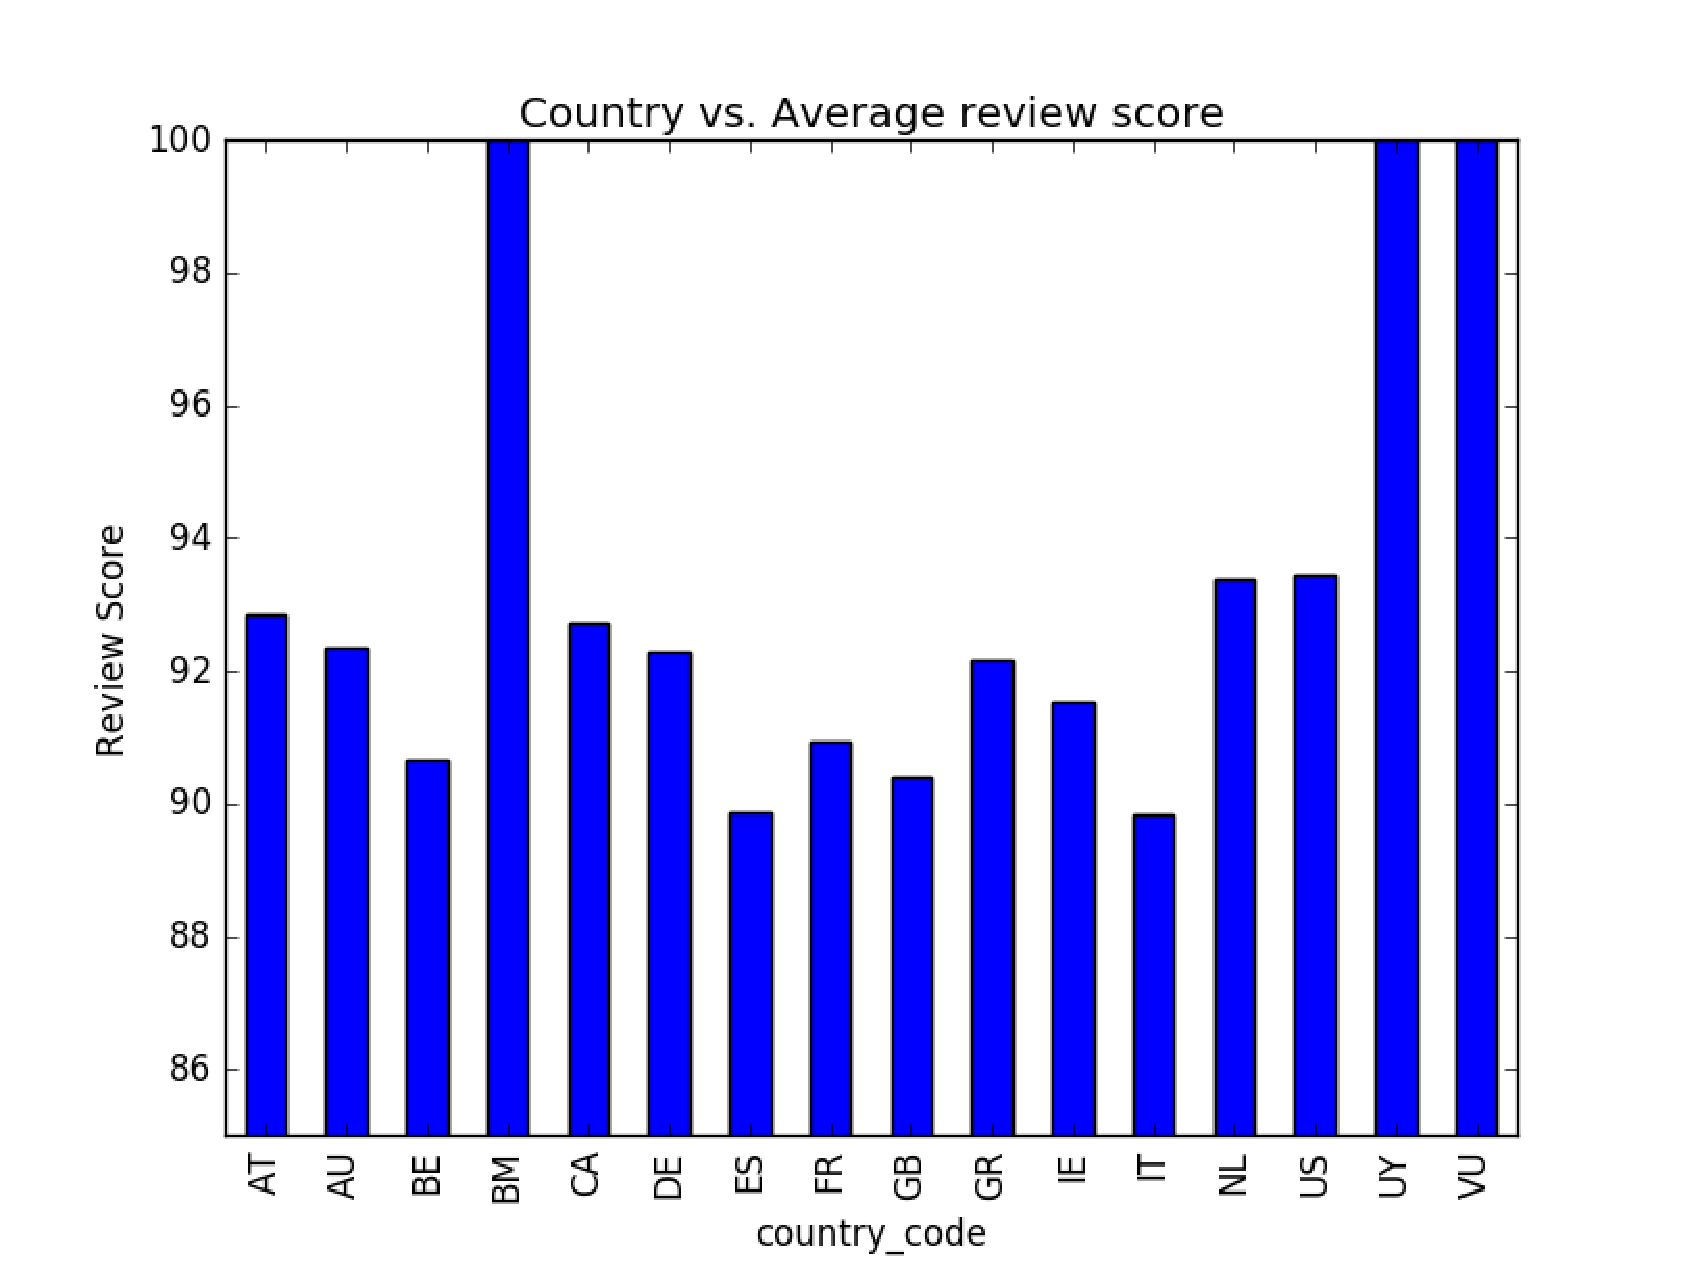
\includegraphics[height=2in, width=3in]{country-avgRating}
\caption{Average rating score distribution among countries}
\end{figure}

When comes to average review scores, most of countries get scores over 90. BM, UY and VU receives average scores of 100, but since the number of listing for these 3 countries in this data set is very limited, it probably has a large bias here. Besides these 3 countries, US and NL are probably best reviewed places to go on Airbnb, IT and ES are the worst reviewed, but still has average scores of over 89.

\FloatBarrier
\section{Proposed Algorithmic Approach}
In this section, we introduce the learning algorithms used to implement the recommendation and evaluate their performances. At first, some basic classifiers are used and compared to find the optimal one for predictions with the lowest error rate. Based on that result, some ensemble technicals such as boosting algorithm, random forest and feature selection are involved to improve the performance. Meanwhile we also use collaborative filtering to build a recommendation model, in which the training dataset is clustered into \emph{k} clusters and each testing instance is label by its closest cluster. A 3-layer ensemble classifier framework is also introduced to achieve performance improvements.

\subsection{Data preprocess}
The original properties for each users involve different data types, includes date and timestamp, so we need to convert all the features into numerical or categorical. As described in Table \ref{table:preprocess}, we compute the lag days between \emph{date\_first\_booking} and \emph{date\_account\_created} and divide the result into four categories [=0, < 0, >0, NA]. Some operation is also taken on \emph{date\_first\_booking} and \emph{timestamp\_first\_active}. For the age attribute, the missing values are replaced by the conditional mean and all the values are scaled by mean and standard deviation. Since the values in \emph{signup\_flow} are integers from 0 to 25, this attribute is considered as categorical when training the model. The training and testing set occupy 80\% and 20\% of entire data set.

\begin{table}[!htb]
\centering
\caption{Data Preprocess}
\label{table:preprocess}
\begin{tabular}{|c|l|} \hline
Processed Attribute & Description\\ \hline
\shortstack{Lag between date\_first\_booking \\ and date\_account\_created} & 
\shortstack[l]{Divided into 4 categories\: \\ =0, <0, >0, NA.}\\ \hline
\shortstack{Lag between date\_first\_booking \\ and timestamp\_first\_active} & 
\shortstack[l]{Divided into 3 categories\: \\ =0, >0, NA}\\ \hline
Age & 
\shortstack[l]{Replace the missing values \\
with the conditional mean; \\
scale the age with mean \\
and standard deviation} \\ \hline
signup\_flow & Categorical Attribute \\ \hline
Others & Original value \\
\hline\end{tabular}
\end{table}


\subsection{Basic and Ensemble Classifiers}
Initially we use \emph{WEKA} package to implement the basic classifiers including Decision Tree, Naive Bayes and Support Vector Machine (SVM). The comparison of error rates shows that C4.5 Decision Tree has the best performance among these classifiers because its error rate is much lower than other classifiers. To verify the results we also implemented the same classifiers in \emph{Scikit Learn} and obtain the error rates based on the training set size as Figure.\ref{fig:basic classifier}. In the basic classifier, Naive Bayes starts at an error rate of 49\% and drops drastically when instance number reaches about 8K. It achieves 70\% accuracy at 50K and has not changed as the size of dataset increases. For Support Vector Machine and Logistic Regression, the error rates remain at around 29\% and have not changed as the number of instances increases. Decision Tree starts at an accuracy rate of 70\% and gradually decreases as the number of instances increases, and finally reaches around 74\% accuracy when the number of instances is 70K.

\begin{figure}[!htb]
\centering
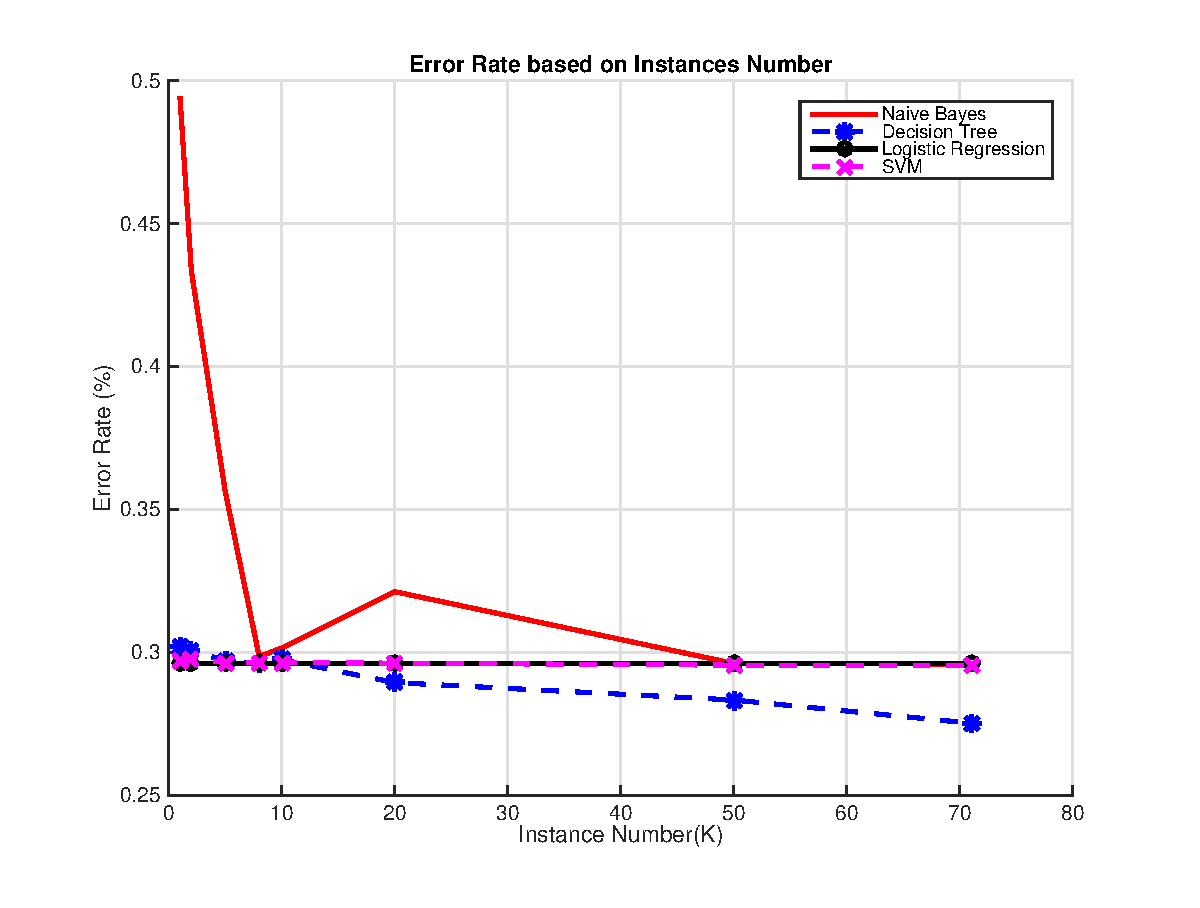
\includegraphics[height=2in, width=3in]{Basic_Classifiers_2}
\caption{Error Rates for Basic Classifier}
\label{fig:basic classifier}
\end{figure}

To improve the performance of the basic classifier, Random Forests and Gradient Boosting with Decision Tree are introduced and have shown improvements in accuracy as Figure.\ref{fig:ensemble classifier} indicated.  The baseline is Decision Tree, which starts at an error rate of 39\% and decreases as the training instances increase. It reaches an error rate of 33\% when the data set is at 70K. Compared to Decision Tree, Random Forests receives about 5\% lower on error rate, starting at 30\% and declining to 27.5\%. Gradient Boosting with Decision Tree shown great performance on the training data, which is initially at 24.5\% and decreases dramatically within the first 5K. Its error rate can achieve 22.5\%, which is much better than Random Forests and any other classifiers.

\begin{figure}[!htb]
\centering
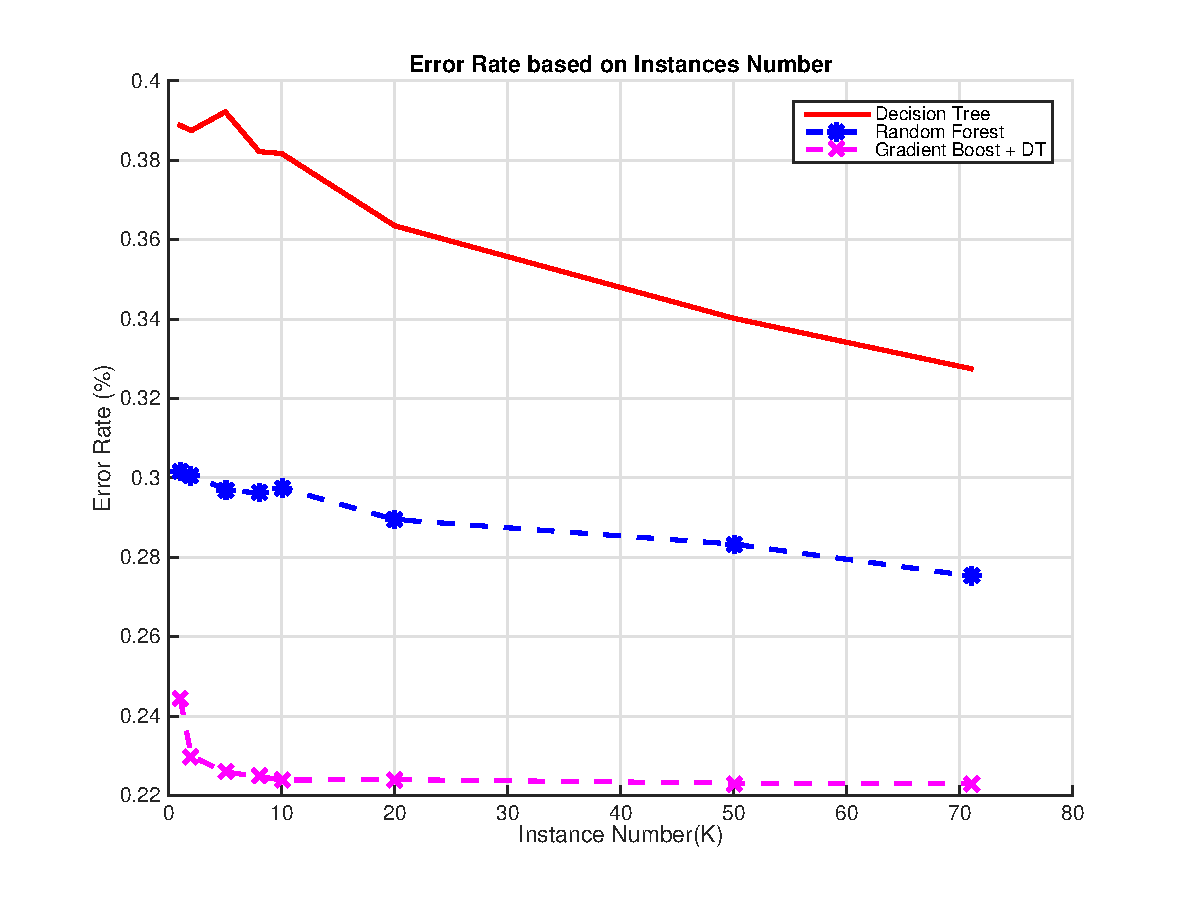
\includegraphics[height=2in, width=3in]{Ensemble_Classifiers_2}
\caption{Error Rates for Ensemble Classifier}
\label{fig:ensemble classifier}
\end{figure}

In order to enhance the accuracy rate further, we also performed feature selection with PCA implemented by \emph{Scikit Learn}. By using feature selection, we hope to eliminate the less relevant information and get a higher accuracy. Among the current 11 features, we use PCA to select 8 features before training the model and obtain the results shown in Figure.\ref{fig:pca}. By comparing to the performance of the original classifiers without PCA, Feature Selection using PCA increases the error rate as the number of instances increase, which suggests that some important information have been dropped. The only exception is Adaboosting with Decision Tree, in which the feature selection cancelled the overfitting.

\begin{figure}[!htb]
\centering
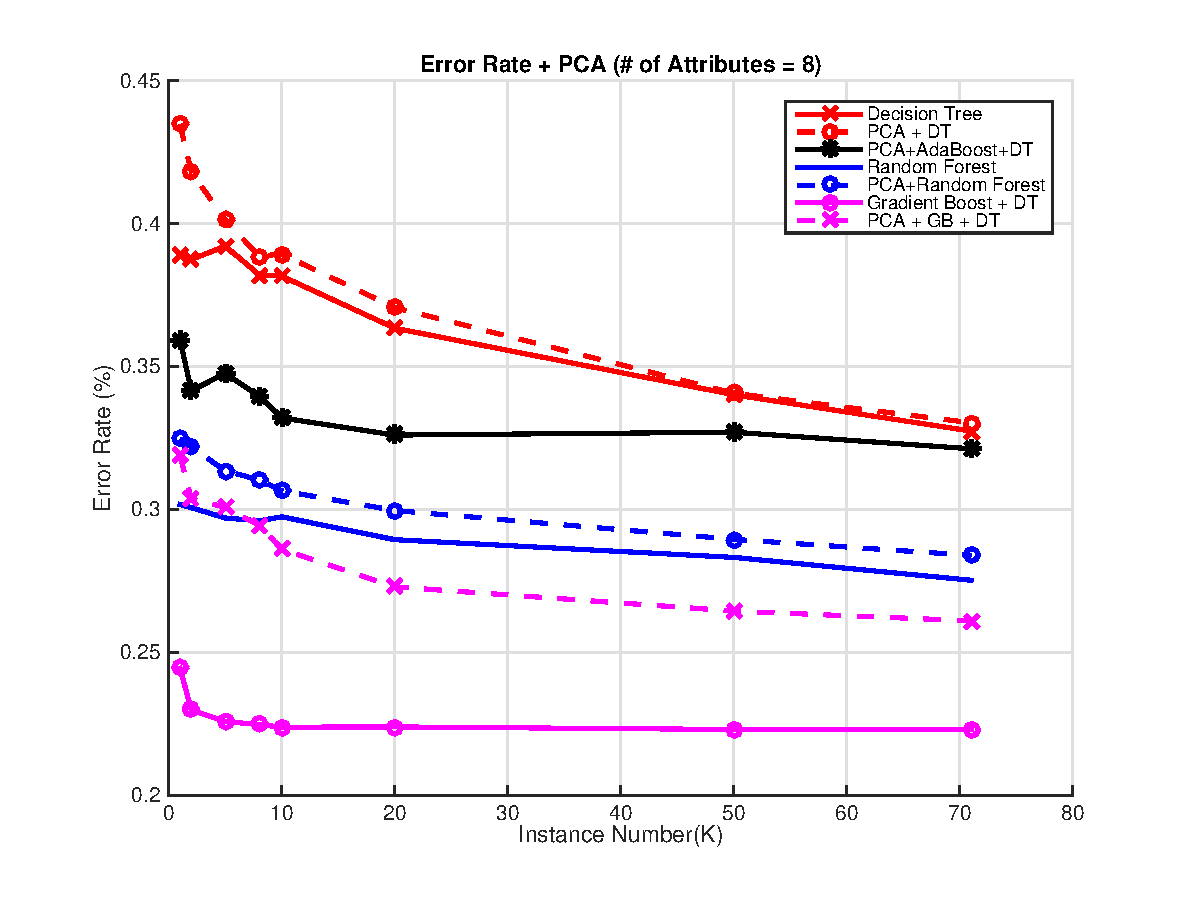
\includegraphics[height=2in,width=3in]{PCA_Classifiers}
\caption{PCA with Classifiers}
\label{fig:pca}
\end{figure}

\subsection{Collaborative Filtering}

To find the optimal recommendation algorithm with the lowest error rate, collaborative filtering is also implemented. In this approach, we consider the \emph{destination\_country} as an attribute and use \emph{k} means to aggregate the similar users based on all the properties. After clustering, each cluster is labeled with the majority destination among all of its members. To evaluate the model, each test case is predicted as the label of its closest cluster. 

The distance between each pair of users is computed by Euclidean Distance, and the Within Group Sum of Square (WGSS) of distance is used as a measurement. In order to find the optimal cluster number, we define a threshold $\epsilon$. When the change rate of WGSS is smaller than the threshold, the best value of \emph{k} is achieved. As Table.\ref{table:clustering} shown, as the threshold becomes smaller, more clusters need to be aggregated and thus a lower rate can be achieved. When $\epsilon$ is 0.001\%, the error rate can achieve 21.37\% which is better than the ensemble classifiers and basic classifiers. The trend of WGSS with the cluster is indicated in Figure.\ref{fig:k means}, where the WGSS falls rapidly until the cluster number is about 400, where the best value of \emph{k} is reached.

\begin{table}[!htb]
\centering
\caption{Clustering Parameters}
\label{table:clustering}
\begin{tabular}{|c|c|c|c|} \hline
\shortstack[l]{Percentage Change \\ of WGSS} & Cluster Num & WGSS & Error Rate \\ \hline
< 0.3\% & 10 & 114013 & 0.3036 \\ \hline
< 0.1\% & 17 & 106895 & 0.2978 \\ \hline
< 0.03\% & 67 & 84909 & 0.2700 \\ \hline
< 0.003\% & 163 & 73112 & 0.2330 \\ \hline
< 0.001\% & 424 & 55412 & 0.2137 \\
\hline\end{tabular}
\end{table}

\begin{figure}[!htb]
\centering
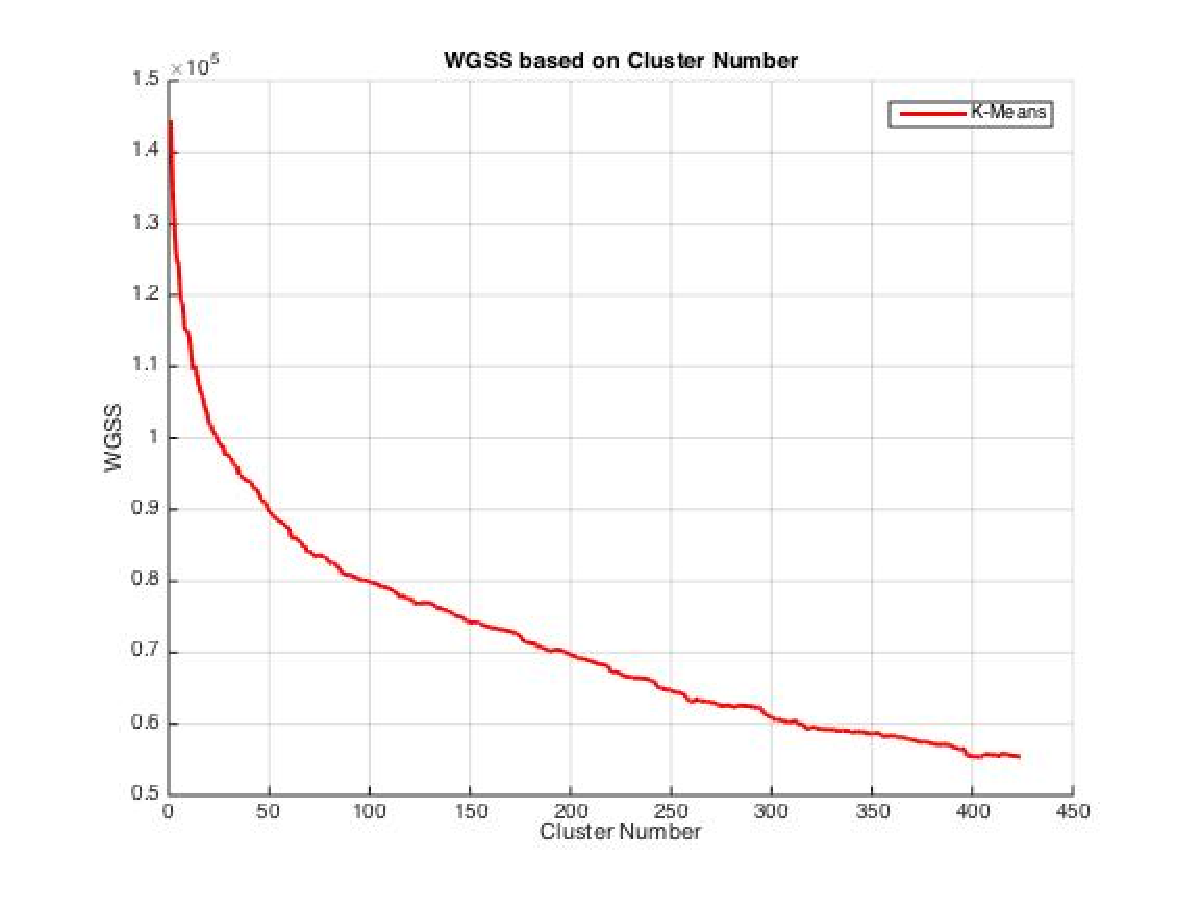
\includegraphics[height=2in,width=3in]{K_Means}
\caption{WGSS based on Clusters}
\label{fig:k means}
\end{figure}

\FloatBarrier
\subsection{Three Layer Ensemble}
In the previous section, results from the basic ensemble methods does not differ significantly from individual classifier results. We then combine different ensemble methods to build this three layer Ensemble methods\cite{3layer}.

First of all, in order to perform multilayer ensemble, we need to partition the dataset into 3 parts: training set 64\%, validation set 16\%, testing set 20\%. From this point on we will use X to denote features or predictions and y to denote labels.

For the first layer, we have used 6 individual classifiers: Logistic Regression, Random Forrest, Gradient Boosting, Decision Tree, Extra Tree, K Nearest Neighbor. All the classifiers have been applied twice. First, classifiers are trained on X\_train, y\_train and are used to predict the class probabilities of X\_valid. Next, classifiers are trained on X = X\_train + X\_valid, y = y\_train + y\_valid and are used to predict the class probabilities of X\_test.

For the second layer, the predictions on X\_valid from first layer are concatenated and used to create a new training set XV, y\_valid. The predictions on X\_test are concatenated to create a new test set XT, y\_test. Then we train two following ensemble methods on XV, y\_valid, and make predictions on XT.

The first ensemble method is denoted as ENA, which computes optimized weights for each prediction X made from first layer classifiers such that it minimizes log\_loss of test result.

The second ensemble method is denoted as ENB. ENB is similar to ENA, but the weights will be assigned with respect to the number of classes we have. For example, X1,X2,...,Xn is the set of predictions given, for each Xi = Xi1,Xi2,...,Xim, where m is the number of classes, and assign weights to each predictions with respect to different classes.

In the end of this layer, we apply a Isotonic Calibrated Classifier obtained from the \emph{Scikit Learn} package in python to generate two new classifiers. Thus we have obtained two ensemble classifiers and two isotonic calibrated classifier in the second layer.

Then comes to the third layer, we assign arbitrary weights to each classifier we obtained from the previous layer, and combine them into a new classifier. After trying few sets of weights, we found weights [2/13, 4/13, 2/13, 5/13] for [ENA, calibrated ENA, ENB, calibrated ENB] has the lowest log loss. We should have tried to test more weight distributions programmatically in order to find the best one, or to incorporate some statistical techniques here for covering wider range of weight distributions, but due to the time limits, this weight distribution is by far the best value for the result.

The final results for each layer are shown in the tables. Noticed that for first layer, Gradient Boosting classifier has produced much better result compared to other classifiers we used in this experiment. Ensemble methods are not suitable here because weight will be assigned heavily to Gradient Boosting Classifier, and other classifiers might get nearly zero weights. As a result, the ensemble methods might not improve a lot from the result of Gradient Boosting classifier. 

The results from second layer prove that for two ensemble methods ENA and ENB, while the log loss decrease for a very small amount, the error rates still remain the same. The Calibrated Ensemble Methods improves a little on the error rate, but also has increased on log loss. When comes to third layer results, it is worth noticing that although the log loss has decreased from 0.875 to 0.872, error rate has increased from 0.2230 to 0.2231, so it's not very clear if this classifier has really improved the result from a single Gradient Boosting classifier.

In the future, we might want to try more classifiers to see if there exists any other independent classifiers that can match with the result from Gradient Boosting classifier, because only then the ensemble methods can take advantage of few different classifiers and produce more precise results.

\begin{table}[ht]
\centering
\caption{Layer one results}
\label{layer1}
\begin{tabular}{|l|l|l|}
\hline
Classifier          & log\_loss & error\_rate \\ \hline
KNN                 & 2.3201224 & 0.2854003   \\ \hline
Gradient Boosting   & 0.8753181 & 0.22308     \\ \hline
Extra tree          & 6.0773485 & 0.3299713   \\ \hline
Random Forest       & 3.7757482 & 0.2752578   \\ \hline
Logistic Regression & 1.1450557 & 0.29605     \\ \hline
DT                  & 8.9571967 & 0.3264777   \\ \hline
\end{tabular}
\end{table}

\begin{table}[ht]
\centering
\caption{Layer two results}
\label{layer2}
\begin{tabular}{|l|l|l|}
\hline
Methods           & log\_loss & error\_rate \\ \hline
EN\_A             & 0.875309  & 0.22308     \\ \hline
Calibrated\_EN\_A & 0.8933696 & 0.2230236   \\ \hline
EN\_B             & 0.875449  & 0.22308     \\ \hline
Calibrated\_EN\_B & 0.8932008 & 0.2230236   \\ \hline
\end{tabular}
\end{table}

\begin{table}[ht]
\centering
\caption{Layer three results}
\label{layer3}
\begin{tabular}{|l|l|}
\hline
log\_loss & error\_rate \\ \hline
0.8726795 & 0.2231927   \\ \hline
\end{tabular}
\end{table}

\FloatBarrier
\section{Conclusion}

Decision tree demonstrates good performance among all the basic classifiers, which might due to the fact that most of attributes are categorical. As a result, decision tree is suitable for this problem. The ensemble methods can improve the performance effectively and Gradient Boosting works better than Random Forests. In this problem, feature selection is less useful since reducing the number of attributes would sacrifice the relevant information. 

The algorithm based on collaborative filtering can achieve lower error rate than both the basic classifiers and ensemble methods. This algorithm is implemented by k means clustering and its performance is highly depended on the number of clusters to be aggregated. To obtain the best value of cluster number, WGSS is involved as an effective measurement.

Three layer ensemble methods are expected to improve its performance by trying different classifiers such that their results can match with the result from Gradient Boosting. A good takeaway is that weight distributions in the third layer should be explored thoroughly to find the best result.

\medskip

\begin{thebibliography}{9}
\bibitem{data mining} Han, J., Kamber, M., and Pei, J. , "Data Mining: Concepts and Techniques", 3rd Edition, 2011.
\bibitem{statistical} Hastie T., Tibshirani R., and Friedman, J. , "The Elements of Statistical Learning: Data Mining, Inference, and Prediction", 2nd Edition, 2009.
\bibitem{analysis} B.M. Sarwarm et al., "Analysis of Recommendation Algorithms for E-Commerce", ACM Conf. Electronic Commerce, ACM Press, 2000, pp.158-167.
\bibitem{collaborative} K. Goldberg et al., "Eigentaste: A Constant Time Collaborative Filtering Algorithm", Information Retrieval J., vol. 4, no. 2, July 2001, pp. 133-151.
\bibitem{clustering} P.S. Bradley, U.M. Fayyad, and C. Reina, "Scaling Clustering Algorithms to Large Databases", Knowledge Discovery and Data Mining, Kluwer Academic, 1998, pp. 9-15.
\bibitem{cf} L. Ungar and D. Foster, "Clustering Methods for Collaborative Filtering", Proc. Workshop on Recommendation Systems, AAAI Press, 1998.
\bibitem{item2item} G. Linden, B. Smith, and J. York, "Amazon.com recommendations: item-to-item collaborative filtering", Internet Computing 7:1, 2003, pp. 76-80.
\bibitem{massive} Leskovec, J., Rajaraman, A., and Ullman, "Mining of Massive Datasets", 2nd Edition, 2004, pp. 307-341.
\bibitem{3layer} Pons, Sandro Vega., "three\_level\_classification\_architecture", Kaggle, 25 Feb 2016. Web. 28 Apr 2016.

\end{thebibliography}
%\balancecolumns % GM June 2007
% That's all folks!
\end{document}
